\documentclass[5pt]{article}
\usepackage{mathptmx,amsmath}
\usepackage{pdfslide2,pause}
\usepackage{eurosym}
\usepackage[portuguese,english]{babel}
\usepackage{kerkis}
\usepackage{colortbl} % used to highlight row or columns of tables. http://www.tug.org/pracjourn/2007-1/mori/mori.pdf
\usepackage[small]{caption} % more option on http://www.dd.chalmers.se/latex/Docs/PDF/caption.pdf
\usepackage[tight,scriptsize]{subfigure}
\usepackage{lastpage}
\usepackage{chngcntr}
\usepackage[absolute,overlay]{textpos}
\usepackage{tabto}
\usepackage{animate}

\usepackage{multicol}
\usepackage{tcolorbox}
\usepackage{booktabs}

%\usepackage{listings}
\captionsetup{labelformat=empty,skip=-0.8cm}

%\lstset{
%    language=Matlab,                % choose the language of the code
%    basicstyle=\ttfamily\tiny,       % the size of the fonts that are used for the code
%    numbers=none,                   % where to put the line-numbers
%    numberstyle=\tiny,              % the size of the fonts that are used for the line-numbers
%    stepnumber=1,                   % the step between two line-numbers. If it's 1 each line will be numbered
%    numbersep=5pt,                  % how far the line-numbers are from the code
%    backgroundcolor=\color{white},  % choose the background color. You must add \usepackage{color}
%    showspaces=false,               % show spaces adding particular underscores
%    showstringspaces=false,         % underline spaces within strings
%    showtabs=false,                 % show tabs within strings adding particular underscores
%    tab=\rightarrowfill,
%    frame=none,	                 % adds a frame around the code
%    tabsize=2,	                   	 % sets default tabsize to 2 spaces
%    captionpos=b,                   % sets the caption-position to bottom
%    breaklines=true,                % sets automatic line breaking
%    breakatwhitespace=false,        % sets if automatic breaks should only happen at whitespace
%    title=\lstname,                 % show the filename of files included with \lstinputlisting; also try caption instead of title
%    escapeinside={\%*}{*)},          % if you want to add a comment within your code
%    morekeywords={ifftshift,fftshift},
%    keywordstyle=\bfseries\color[rgb]{0,0,0.3},
%    commentstyle=\color[rgb]{0.133,0.5,0.133}
%}
%\lstset{
%    emph={function,end,for,if,while},
%    emphstyle=\bfseries\color[rgb]{0.6,0,0},
%}

\definecolor{itblue}{rgb}{0.0,0.0,0.5}
\definecolor{itred}{rgb}{0.82,0.18,0.24}
\newcommand{\pageNum}{
    \begin{picture}(0,0)(0,0)
        \put(-15,-390){
            \begin{minipage}{1.8cm}
            \end{minipage}
        }
    \end{picture}
}
\newcommand{\cb}[1]{{\color{itblue} #1}}%
\newcommand{\cred}[1]{{\color{itred} #1}}%
\newcommand{\bb}[1]{{\textbf{\color{itblue} #1}}}%
\newcommand{\br}[1]{{\textbf{\color{itred} #1}}}%
\renewcommand{\labelitemi}{\textcolor{itred}{\normalsize $\bullet$}}
\renewcommand{\labelitemii}{\textcolor{itblue}{$\bullet$}}
\newcommand{\mysection}[1]{\section*{\pageNum\color{itred}\sffamily #1}\vspace*{0.5cm}\overlay{it_1.png}\sffamily}%
\newcommand{\ITfootnote}[1]{\hspace{1.8cm}\begin{minipage}{13cm}\tiny{#1}\end{minipage}}
\newcommand{\edfaGain}{$G=\exp\left(\frac{\alpha}{2}L_{span}\right)$}
\newenvironment{reference}{
    \begin{textblock*}{0.7\textwidth}(32mm,137mm)\tiny\noindent\bgroup\color{black}
}
{
    \egroup\end{textblock*}
}


\graphicspath{{./Figures/}}
\pagestyle{title}

\hyphenpenalty=50000
\tolerance=10000

\setlength{\textheight}{1.5\textheight}

%%%%%%%%%%%%%%%%%%%%%%%%%%%%%%%%%%%%%%%%%%%%%%%%%%%%%%%%%%%%%%%%%%%%%%%%%%%%%%%%%%%%%%%%%%%%%%%%%%%
%%%%%%%%%%%%%%%%%%%%%%%%%%%%%%%%%%%%%%%%%%%%%%%%%%%%%%%%%%%%%%%%%%%%%%%%%%%%%%%%%%%%%%%%%%%%%%%%%%%

\begin{document}

%************************************************************************************************
%                                          SLIDE
%************************************************************************************************
\pagenumbering{roman}
\begin{titlepage}  \overlay{it_0.png}

\color{itblue} \sffamily \noindent \small
\hspace*{1cm}  Universidade de Aveiro\\ %Instituto\\ Superior T�cnico, Instituto de Telecomunica��es\\
\hspace*{1cm}  2017-2018\\ %Lisboa, 14th of February, 2013\\

\vspace*{1cm}
\begin{center}
    \color{black} \sffamily \noindent \Large
    \br{Simplified Coherent Transceivers for Optical Communication Networks\\}
\end{center}
\vspace{6mm}
\begin{center}
    \color{black}
    \textbf{Romil Patel\\}
    {(romilkumar@ua.pt)}
\end{center}

\vspace{0.0mm}
\scriptsize
\begin{center}
Department of Electronics, Telecommunications and Informatics,\\
University of Aveiro, Aveiro, Portugal\\
Instituto de Telecomunica\c{c}\~{o}es, Aveiro, Portugal\\
\end{center}

\vspace{1.0cm}
\hspace*{13.2cm}\tiny \copyright 2005, it - instituto de telecomunica\c{c}\~{o}es\hfill

\end{titlepage}


\renewcommand{\headsep}{-25pt}
\pagenumbering{arabic}



%--------------------------------------------------------------------------------------------------
%------------ SLIDE-------
\mysection{Theocratical Overview}\large
\vspace{0cm}

\begin{itemize}
  %\item Coherent optical transmission schemes are optimal from the stand point of spectral efficiency since they allow the encoding of information in both quadrature and polarization.
  \item Coherent optical schemes require two optical hybrids and four pairs of balanced photodetector. It formulate a solution for medium-to-long-reach applications, however, cost of such receiver become an obstacle in short reach application like PON, inter-data-center communications and metropolitan network.
  \item Kramers-Kronig transceiver provides a solution for such short links. It allows the reconstruction of complex constellation from an intensity measurement using a single-photo-diode.
  \item The kramers-Kronig scheme relies on identifying a condition which ensures that the received signal is minimum phase.
  \item The following few slides would give a comprehensive overview about the working principle Kramers-Kronig receiver.

\end{itemize}

%--------------------------------------------------------------------------------------------------
%------------ SLIDE--------------------------------------------------------------------------------

%--------------------------------------------------------------------------------------------------
%------------ SLIDE--------------------------------------------------------------------------------

%--------------------------------------------------------------------------------------------------
%------------ SLIDE-------
\mysection{1. What is minimum phase signal?}\large
\begin{itemize}
  \item A necessary and sufficient condition for a complex signal \textbf{$A(t)=A_{s}(t)+\bar{A}$} to be minimum phase is that the curve described in a complex plane by $A(t)$ when $t\rightarrow -\infty$ to $t\rightarrow \infty$ \textbf{does not encircle the origin}.\\
      where, $A_{t}\rightarrow $ Single sideband (SSB) signal \& $\bar{A}\rightarrow$ DC value.
      
  \item A minimum-phase signal has an useful property that the \textbf{natural logarithm }of the magnitude  related to the phase angle by the Hilbert transform.
\end{itemize}
\begin{figure}[hbt]
	\centering
	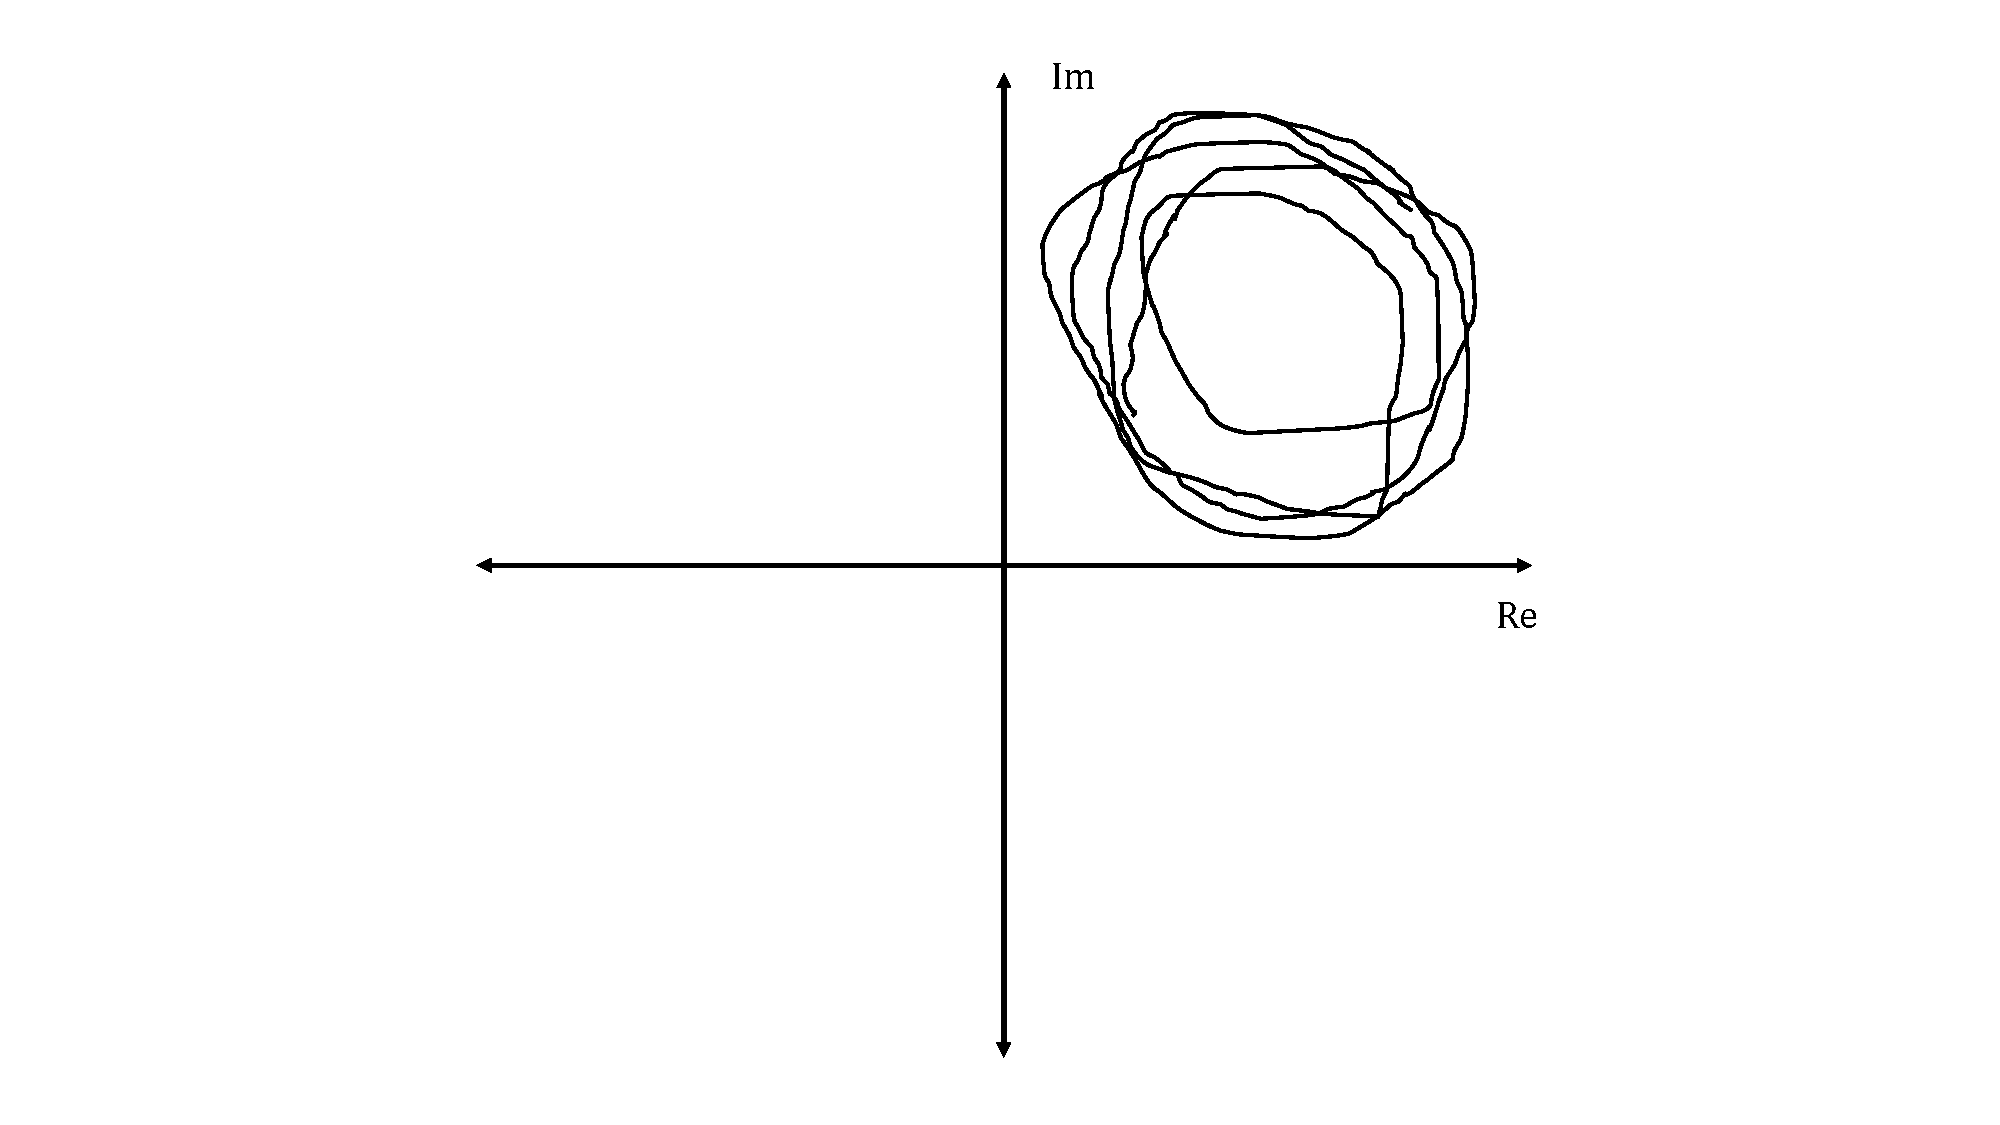
\includegraphics[width=0.5\textwidth, height=5cm]{./figures/MP_Signal.pdf}
    \vspace{5mm}
    \caption{Minumum Phase Signal}\label{}
\end{figure}

%--------------------------------------------------------------------------------------------------
%------------ SLIDE-------
\mysection{2. How we can use these signals and profit from them?}\large
\begin{itemize}
  \item \textbf{SSB Signal:}\\
         If we denote a SSB signal $A_s(t)$ as,
        \begin{equation}
        A_s(t)=A_{s,r}(t)+iA_{s,i}(t)
        \label{Eq:5.31}
        \end{equation}
        then in the equation \ref{Eq:5.31}, the real and imaginary parts $A_{s,r}(t)$ and $A_{s,i}(t)$ are related through the Kramers-Kronig relation with each other as,
\begin{equation}
\begin{split}
A_{s,r}(t) &=-\frac{1}{\pi} p.v. \int_{-\infty}^{\infty} \frac{A_{s,i}(t')}{t-t'} dt' \\
A_{s,i}(t) &=\frac{1}{\pi} p.v. \int_{-\infty}^{\infty} \frac{A_{s,r}(t')}{t-t'} dt' \\
\end{split}
\label{Eq:5.38}
\end{equation}



\end{itemize}


%--------------------------------------------------------------------------------------------------
%------------ SLIDE-------
\mysection{}\large
\vspace{0cm}
\begin{tcolorbox}	
	\begin{tabular}{p{1cm} p{0.2cm} p{15cm}} 	
		\textbf{Note}&:& Single sideband signal is the frequency translated version of an analytical signal as,\\
		\textbf{}	 & & $A_s(t)=Re\{[s(t)+i\hat{s}(t)] e^{i2\pi f_0 t}\}$\\
	\end{tabular}
\end{tcolorbox}
\begin{itemize}
\item \textbf{Minimum Phase Signal:}\\
    Given function $A(t)=A_{s}(t)+\bar{A}$ never encircles the origin for $t\in(-\infty,\infty)$.
\begin{equation}
G(t)=ln\bigg[\dfrac{A(t)}{\bar{A}}\bigg]\\
\label{Eq:A1}
\end{equation}

Under the hypothesis of signal being minimum phase, the phase information can be reconstructed by from its intensity as,
\begin{equation}
\begin{split}
\phi(t) &= \bar{\phi} + \frac{1}{2\pi} p.v. \int_{-\infty}^{\infty} \frac{ln|A(t)|^2}{t-t'} dt'\\
\end{split}
\label{Eq:E1}
\end{equation}
\end{itemize}


%--------------------------------------------------------------------------------------------------
%------------ SLIDE-------
\mysection{Simulation setup}\large
\begin{itemize}
  \item \textbf{Transmitter setup}
  \begin{figure}[hbt]
	\centering
	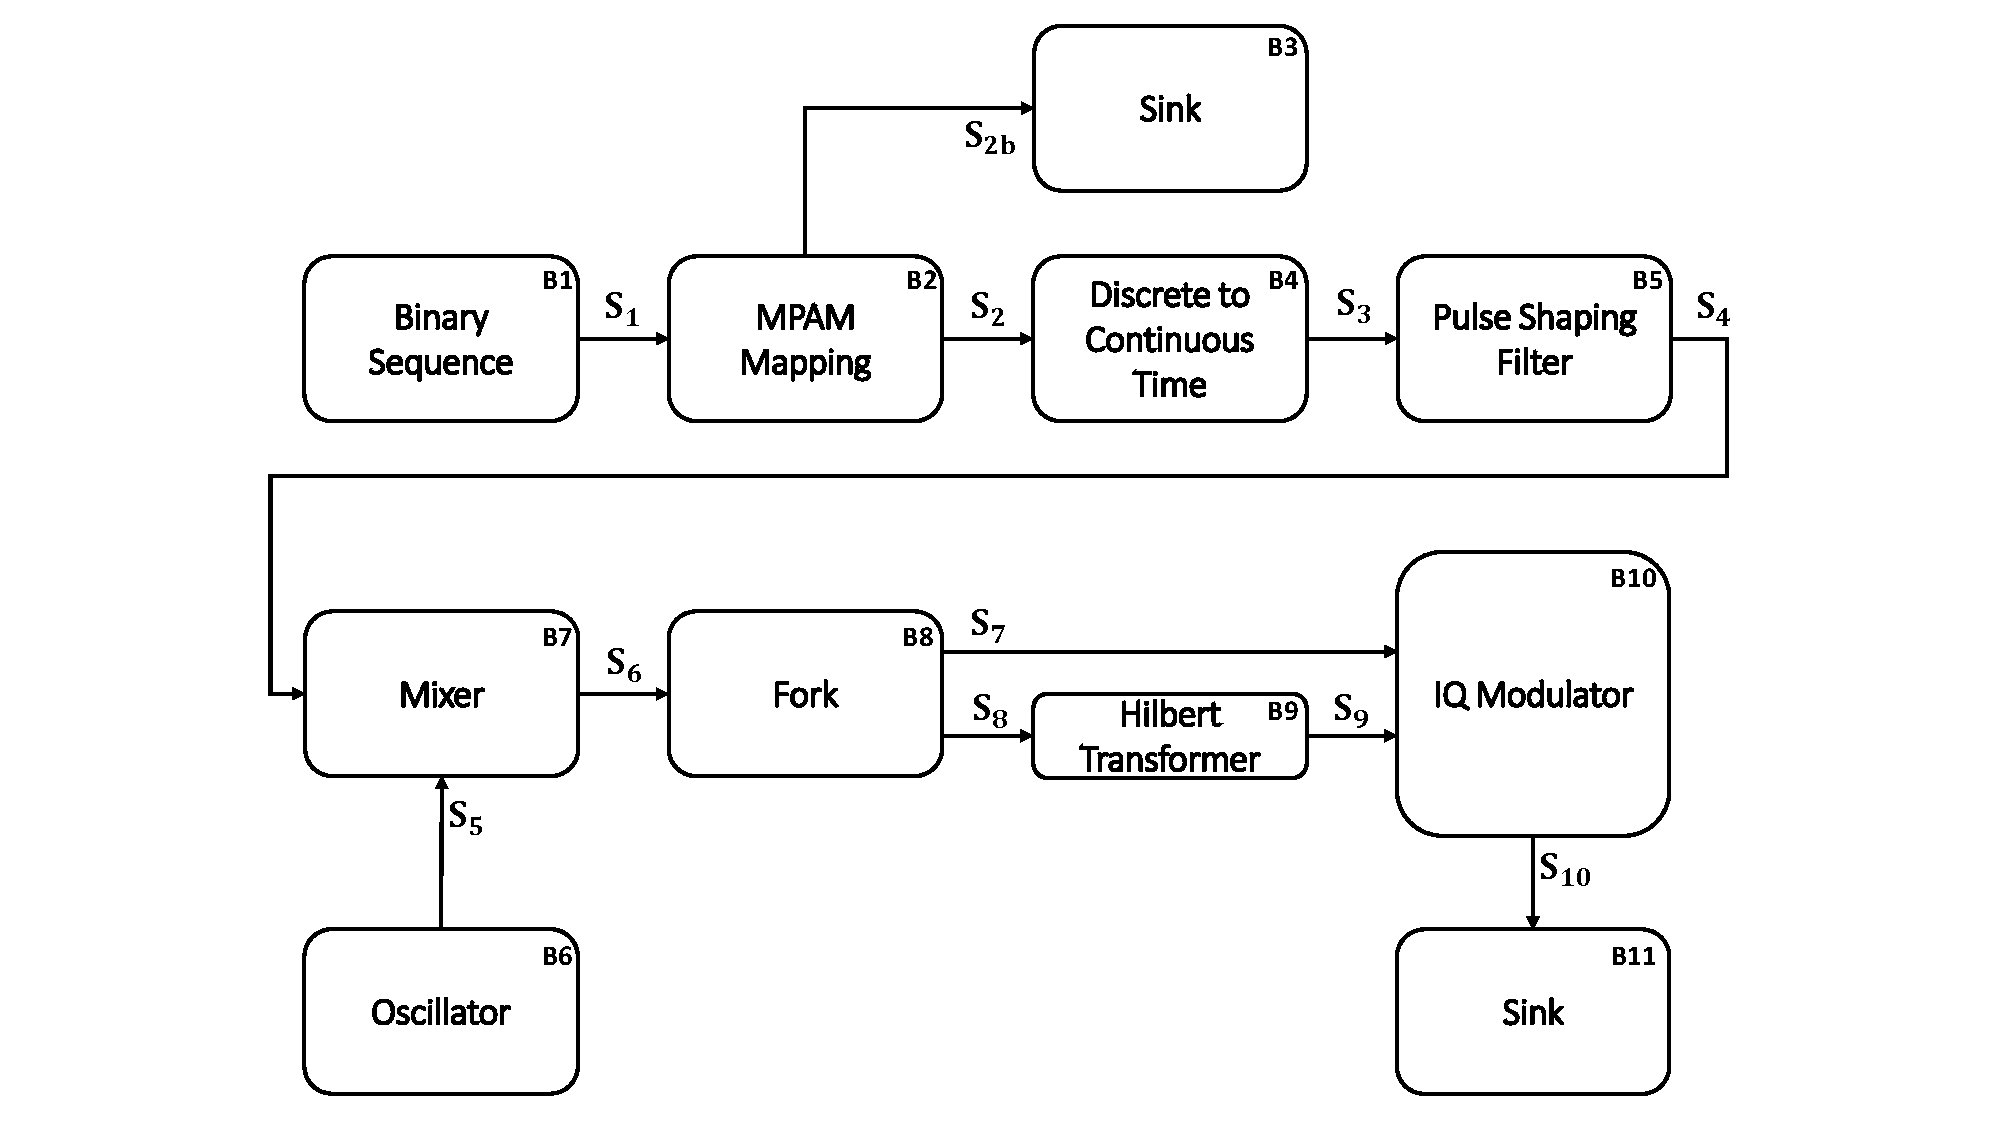
\includegraphics[width=1.0\textwidth, height=10cm]{./figures/Simulation_setup_Tx.pdf}
    \vspace{3mm}
    \caption{Transmitter simulation setup}\label{}
\end{figure}
\end{itemize}
%--------------------------------------------------------------------------------------------------
%------------ SLIDE-------
\mysection{Simulation Results}\large
  \begin{figure}[hbt]
	\centering
	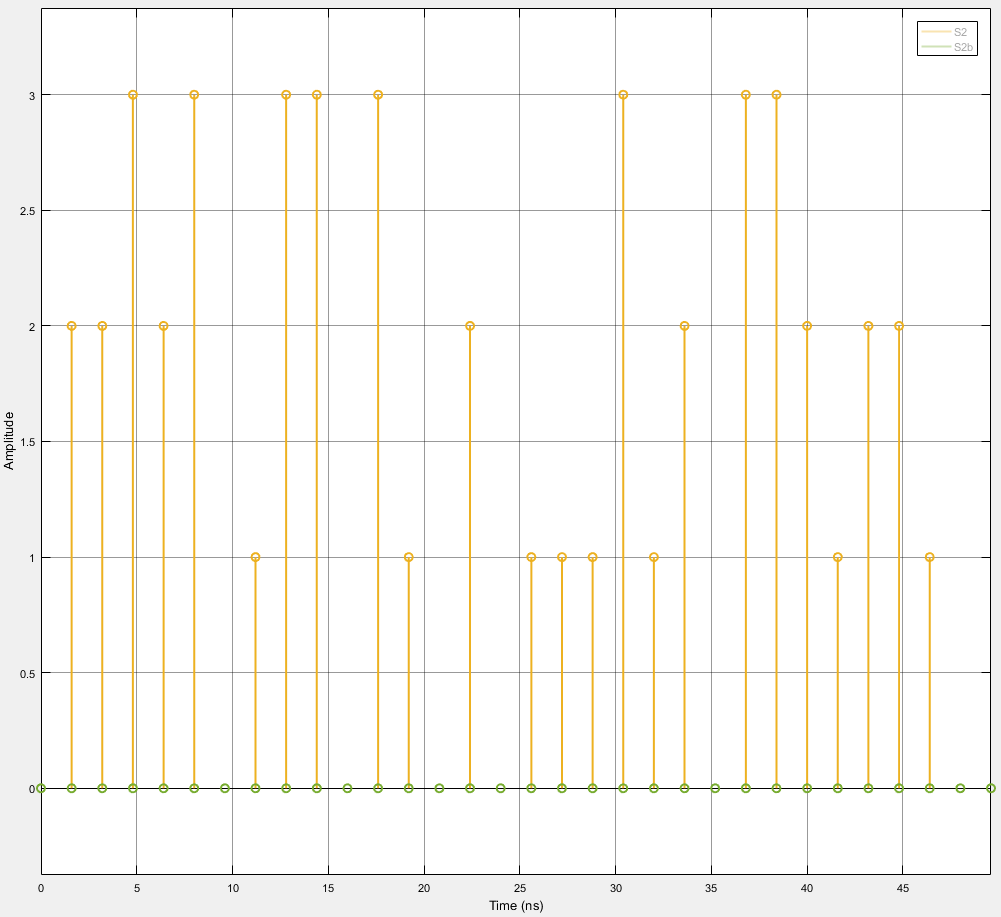
\includegraphics[width=0.85\textwidth, height=10cm]{./figures/S2S2b.png}
    \vspace{10mm}
    \caption{S2 and S2b signals}\label{}
\end{figure}

\mysection{}\large
  \begin{figure}[hbt]
	\centering
	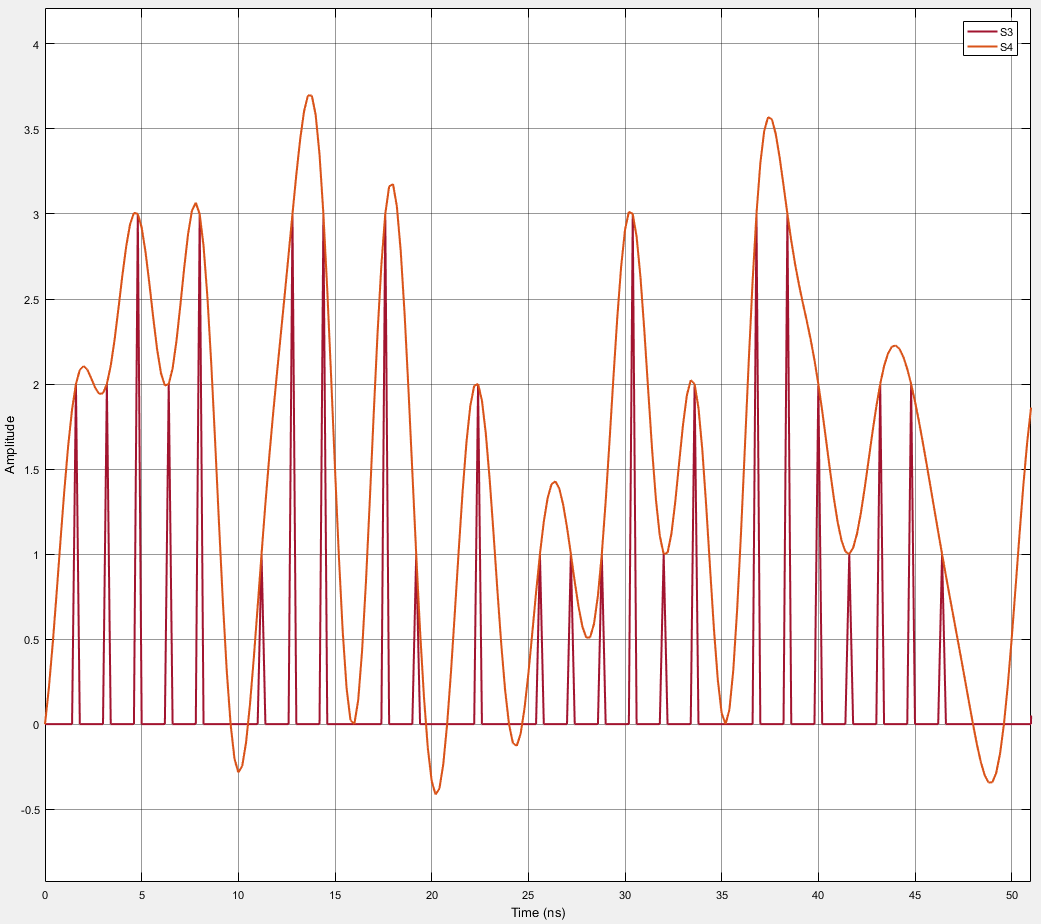
\includegraphics[width=0.85\textwidth, height=10cm]{./figures/S3S4.png}
    \vspace{10mm}
    \caption{S3 S4 signals}\label{}
\end{figure}

\mysection{}\large
  \begin{figure}[hbt]
	\centering
	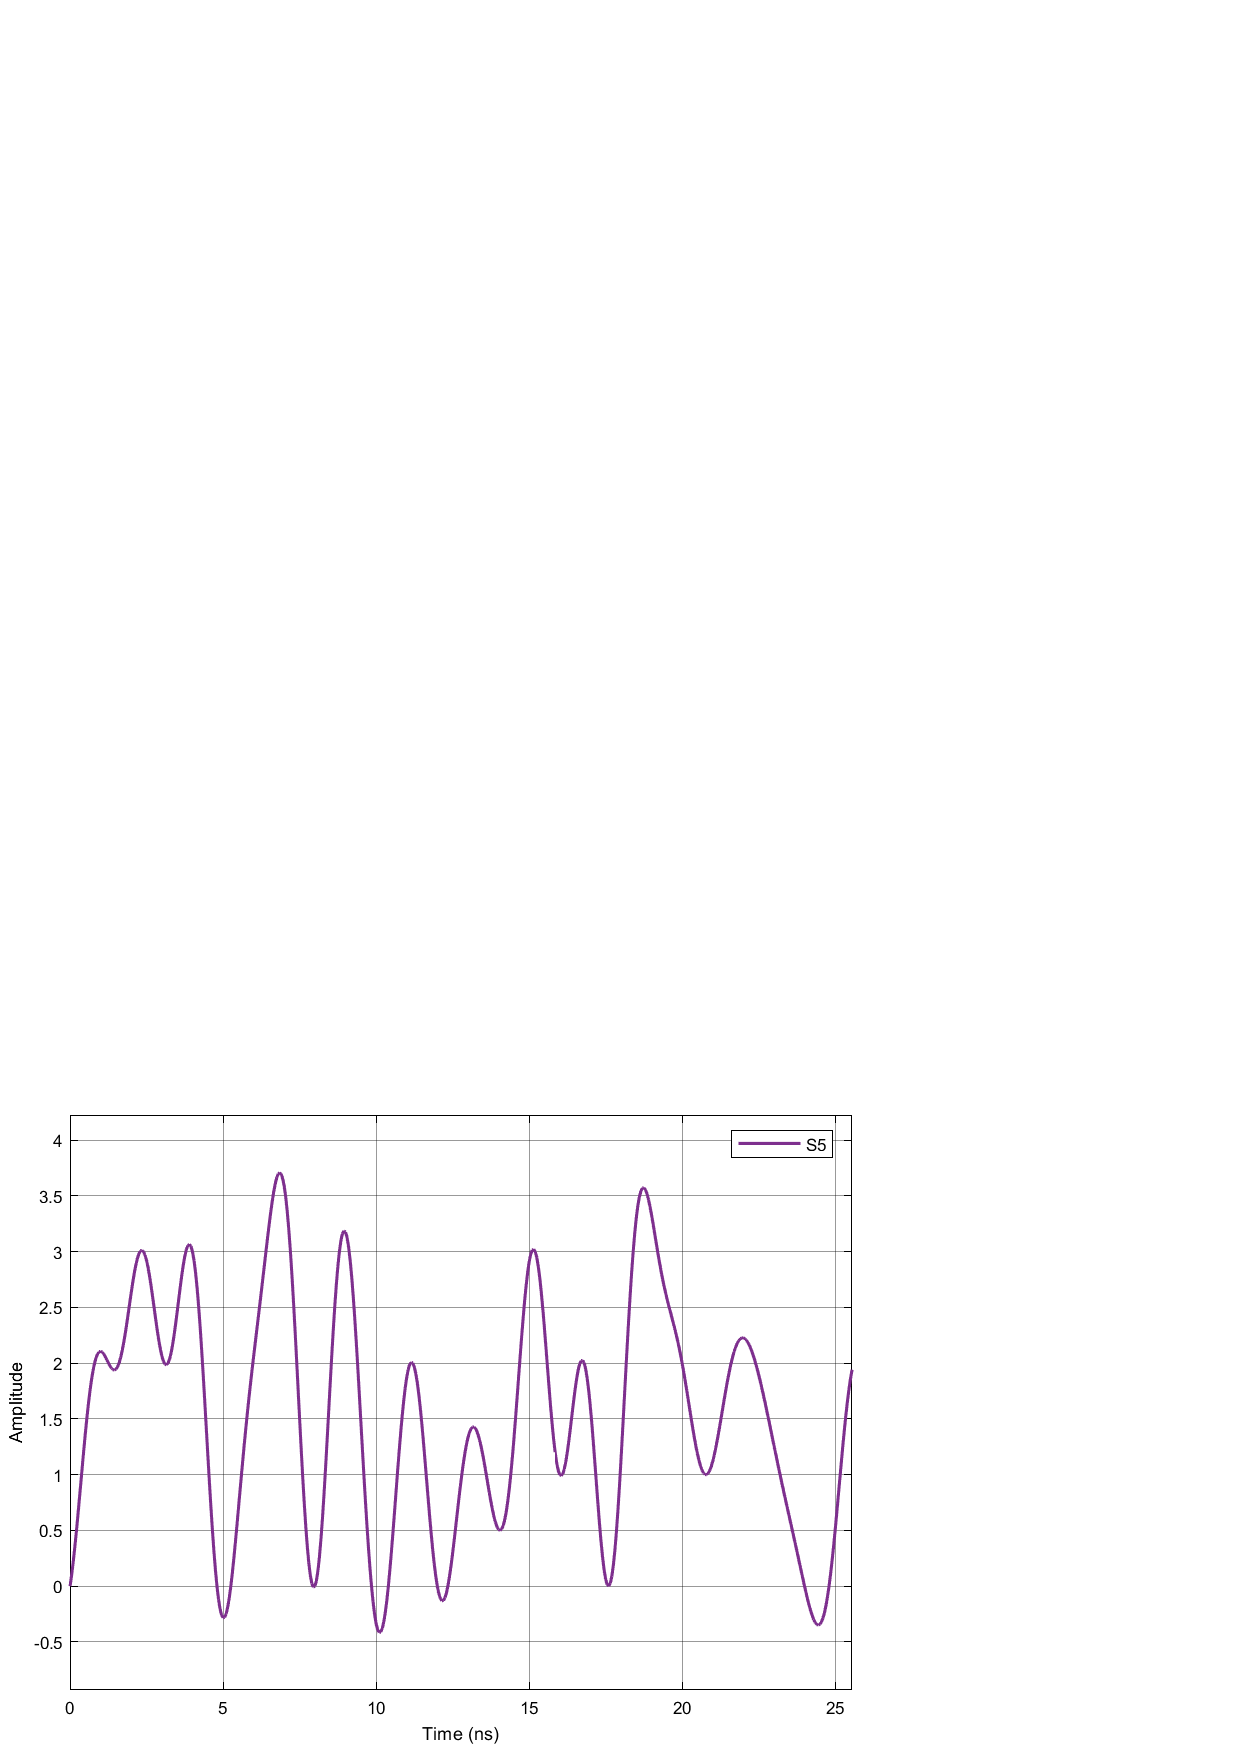
\includegraphics[width=0.85\textwidth, height=10cm]{./figures/S5.png}
    \vspace{10mm}
    \caption{S5 signal}\label{}
\end{figure}

\mysection{}\large
  \begin{figure}[hbt]
	\centering
	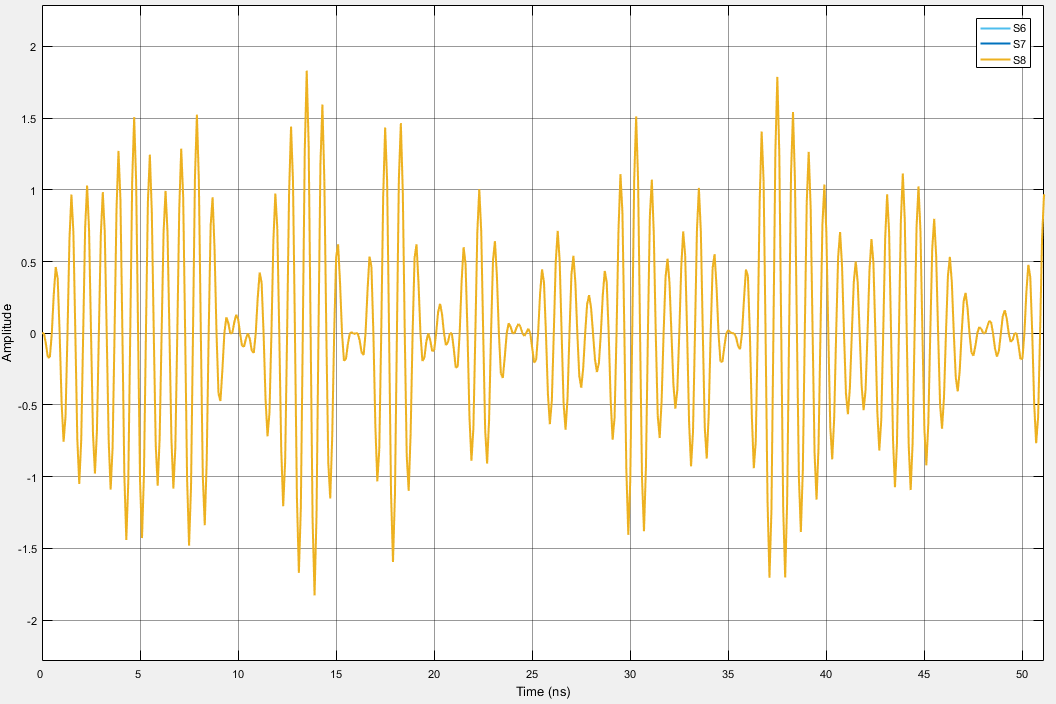
\includegraphics[width=0.85\textwidth, height=10cm]{./figures/S6S7S8.png}
    \vspace{10mm}
    \caption{S6, S7 and S8 signals}\label{}
\end{figure}
%--------------------------------------------------------------------------------------------------
%------------ SLIDE-------
\mysection{Experimental setup}\large
\begin{itemize}
  \item \textbf{Envisioned lab setup}
  \begin{figure}[hbt]
	\centering
	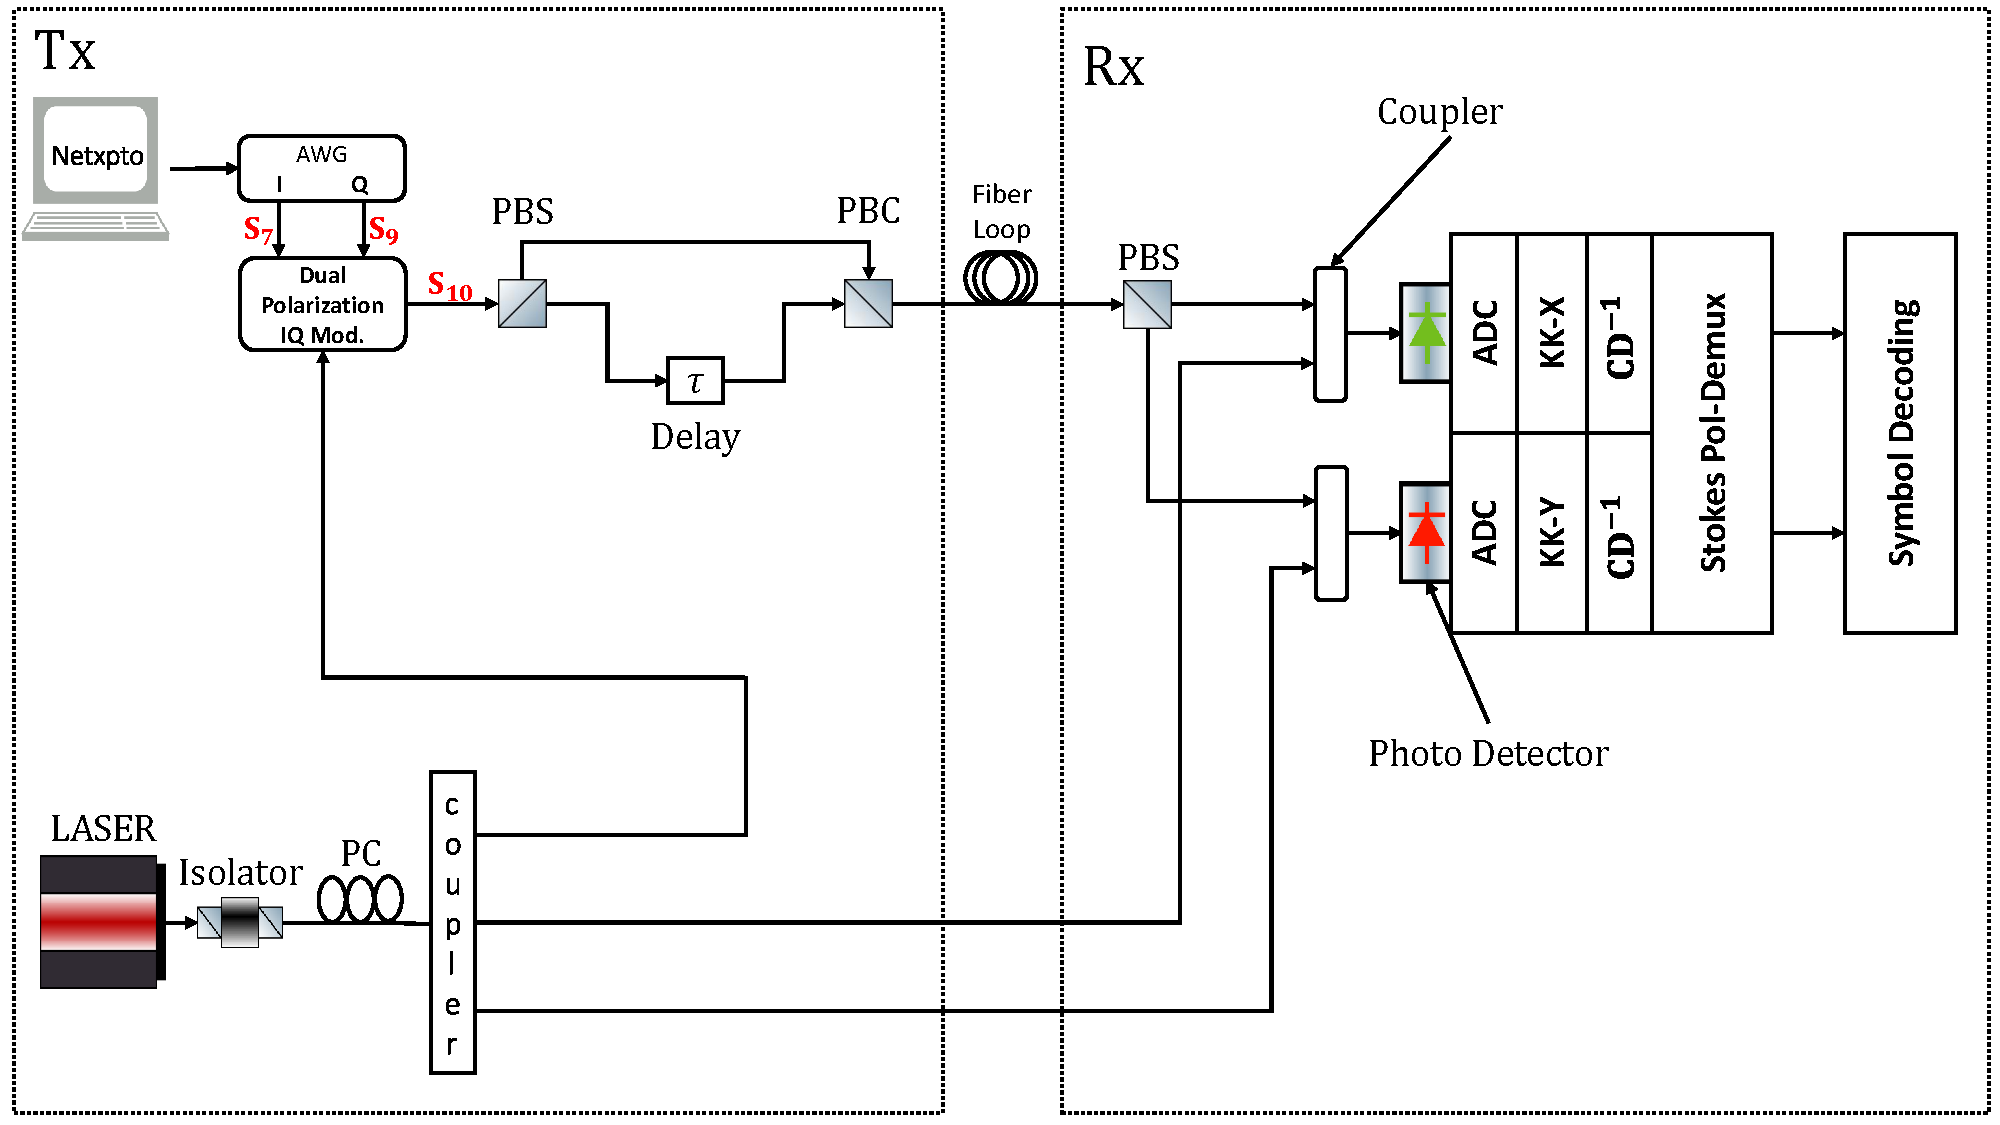
\includegraphics[width=1.0\textwidth, height=10cm]{./figures/Practical_setup_TxRx.pdf}
    \vspace{3mm}
    \caption{PDM Kramers-Kronig receiver experimental setup}\label{}
\end{figure}
\end{itemize}

%-------------------------------------------------------------------
%------------ SLIDE ------------------------------------------------
\mysection{} \sffamily
\vspace{-10mm}
\large\centerline{E-mail: romilkumar@ua.pt}


\end{document}
